\documentclass[a4paper]{article}
\usepackage[french]{babel}
\usepackage{amssymb}
\usepackage[dvips]{graphicx}
\newcommand{\dashlinestretch} {}

%------------------------------------------------------------------------------
% Use a small font for the verbatim environment
\makeatletter  % makes '@' an ordinary character
\renewcommand{\verbatim@font}{%
  \ttfamily\footnotesize\catcode`\<=\active\catcode`\>=\active%
}
\makeatother   % makes '@' a special symbol again
%------------------------------------------------------------------------------
\usepackage[headings]{fullpage}
\advance\hoffset by -3mm  % A4 is narrower.
\advance\voffset by  8mm  % A4 is taller.
%END LATEX
%------------------------------------------------------------------------------
%---------- Entete de feuille ----------
\def\entete{D\'etection de contour dans un fichier BMP
\centerline{\bf \large  IUC}
\smallskip
\hrule
\medskip}
\newtheorem{definition}{D\'efinition}
%----------- D\'efinition exercice -------
\newcounter{exerc}
\newcommand{\exercice}{\stepcounter{exerc}
  \setcounter{quest}{0}
  \paragraph{\large \bf Exercice \theexerc~:}}
\newcounter{quest}
\newcommand{\quest}{\stepcounter{quest}
  \setcounter{subquest}{0}
  {\noindent \bf Q \thequest~. }}
\newcounter{subquest}
\newcommand{\subquest}{\noindent \stepcounter{subquest}
  \hspace{0.2cm}{Q \thequest.\thesubquest.~}}

% ---------- C'est parti ---------------

\title{D\'etection de contour dans un fichier BMP}
\author{A.~Sedoglavic \\
Universit\'e des Sciences et Technologies de Lille}
\date{2004--2005}
\begin{document}
\maketitle
\section{Pr\'esentation}

Le but de ce projet sera de d\'etecter des contours dans une image
stock\'ee en BMP\@.  Pour ce faire, nous allons tout d'abord
pr\'esenter le format de fichier
BMP\footnote{http://www.wotsit.org/filestore/bmpfrmat.zip}. Puis, nous
pr\'esenterons la notion de bruitage al\'eatoire d'une image qui
constituera la premi\`ere partie du projet et une m\'ethode de
d\'etection de contour qui constituera la seconde.

\section{Directives concernant la remise de vos projet}
Votre projet devra me parvenir par courriel \`a l'adresse
\verb?sedoglav@lifl.fr? au plus tard le vendredi~$29$ avril~$2005$ minuit~;
le sujet de votre message devra commencer par \verb?[IUPM1 -- PROJET]?
et comporter vos noms.

Votre projet devra \^etre remis sous la forme d'une archive tar
compress\'ee d'extension .tgz comprenant~:
\begin{itemize}
\item un fichier Readme documentant votre projet (auteurs, courriels,
  date, limitation \'eventuelle, etc.)~;
\item une documentation succinte de vos ex\'ecutables (soit sous la
  forme du manuel unix, soit un affichage lors de l'appel de ces
  derniers avec l'option \verb?--help?)~;
\item les fichiers sources (extension .c et .h) constituant votre
  projet~;
\item un fichier Makefile permettant de construire deux  ex\'ecutables~:
  \begin{itemize}
  \item un \textit{bruiteur} suivant les consignes de la
    section~\ref{sec:bruiteur}~;
  \item un d\'etecteur de contour suivant les consignes de la
    section~\ref{sec:contour}~;
  \end{itemize}
  \`a partir des fichiers sources.
\end{itemize}
Cette archive ne devra contenir aucun r\'epertoire et le Makefile
permettre la compilation de vos ex\'ecutable par la seule commande
\verb?make? dans un shell.

Le nom du fichier archive sera n\'ecessairement au format
ProjetIUPM105\_nom1\_nom2.tgz~; nom1 et nom2 \'etant les noms des deux
\'etudiants de votre bin\^ome (si vous \^etes seul, laissez le second
nom vide).
\section{Le format BMP 24 bits non compress\'e}

Nous nous occuperons uniquement dans cette section des fichiers BMP
\emph{non compress\'es} et en \emph{24 bits} puisqu'il s'agit du format
le plus simple \`a manipuler.

Afin d'obtenir ce type de format \`a partir d'une image sous un autre
format, vous pouvez utilisez un utilitaire comme gimp (fonction Save
as) qui peut aussi vous servir \`a visualiser les fichiers BMP produit
par vos codes.

Le fichier est constitu\'e de deux parties distinctes~: l'ent\^ete (le
\emph{header}) et les \emph{donn\'ees non compress\'ees}.

\subsection{Ent\^ete d'un fichier~BMP}

L'ent\^ete est une repr\'esentation binaire des informations
concernant une image. Cette ent\^ete contient des informations sur la
taille de l'image en largeur et en hauteur (en \emph{pixels}), le
nombre de couleurs ou encore le type d'encodage des donn\'ees.

C'est gr\^ace \`a cette ent\^ete que nous allons pouvoir d\'eterminer
si les informations d'un fichier BMP sont conformes \`a ce que l'on
attend en entr\'ee de notre projet.

L'ent\^ete est constitu\'ee d'une s\'erie d'entiers, cod\'es sur 16 ou
32 bits (respectivement 2 ou 4 octets). Ces entiers sont dispos\'es
dans un ordre pr\'ecis :
$$
\begin{tabular}{|l|c|l|}
\hline
&&\\
Nom du champs & Longueur en octets & Signification\\
&&\\
\hline
Identifier      & 2     & Contient toujours  l'octet `B' suivit de l'octet `M'\\
FileSize        & 4     & Taille totale du fichier en octets\\
Reserved        & 4     & Champs r\'eserv\'e, doit \^etre \'egal \`a 0\\
DataOffset      & 4     & Nombre d'octets s\'eparant le d\'ebut du fichier des donn\'ees de l'image\\
HeaderSize      & 4     & Taille en octets de l'header\\
Width           & 4     & Largeur de l'image en pixels\\
Height          & 4     & Hauteur de l'image en pixels\\
Planes          & 2     & Nombre de plans\\
BitsPerPixels   & 2     & Nombre de bits n\'ecessaires pour repr\'esenter un pixel\\
Compression     & 4     & Type de compression\\
BitmapDataSize  & 4     & Taille en octets des donn\'ees de l'image\\
HResolution     & 4     & R\'esolution horizontale de l'image en pixels par m\`etre\\
VResolution     & 4     & R\'esolution verticale de l'image en pixels par m\`etre\\
Colors          & 4     & Nombre de couleurs dans l'image\\
ImportantColors & 4     & Nombre de couleurs importantes\\
\hline
\end{tabular}
$$

Tous les champs ne nous concernent pas ; seuls les champs
$\mathtt{Identifier}$, $\mathtt{DataOffset}$, $\mathtt{Width}$,
$\mathtt{Height}$, $\mathtt{BitsPerPixels}$, $\mathtt{Compression}$ et
$\mathtt{BitmapDataSize}$ nous seront r\'eellement n\'ecessaires.

\exercice\ \\
D\'efinissez un type \texttt{BMP\_Header\_t} contenant toutes les
informations d'une ent\^ete BMP. \'Ecrivez ensuite une fonction
permettant de lire l'ent\^ete d'un fichier BMP, et dont le prototype
sera~:

\begin{verbatim}
    BMPHeader_t *loadBMPHeader(FILE *fichier);
\end{verbatim}

On consid\`ere donc que le fichier \`a donc \'et\'e ouvert \`a
l'ext\'erieur de la fonction, et que le pointeur retourn\'ee par une
fonction \verb|fopen| est donn\'ee en param\`etre (pointeur
\verb|fichier|). La fonction aura pour but de remplir la structure
point\'ee par la valeur de retour et elle retournera~$0$ si
l'op\'eration ne s'est pas effectu\'ee normalement.

\exercice\ \\
\'Ecrivez une fonction permettant de v\'erifier la validit\'e d'une ent\^ete
de fichier BMP\@. La fonction devra v\'erifier~:
\begin{itemize}
\item qu'il s'agit bien d'un fichier BMP (en v\'erifiant que les deux
  premiers octets soient bien `B' et `M')~;
\item qu'il s'agit d'un fichier non compress\'e (le
  champs~$\mathtt{Compression}$ doit \^etre \'egal \`a~$0$)~;
\item que le fichier est bien un fichier en~$24$ bits (le
  champs~$\mathtt{BitPerPixels}$ doit \^etre \'egal \`a~$24$)~;
\item que la taille des donn\'ees ($\mathtt{BitmapDataSize}$) est bien
  \'egal \`a~${\mathtt{Width} \times \mathtt{Height} \times 3}$.
\end{itemize}

Le prototype de la fonction sera le suivant :
\begin{verbatim}
          int isBMPHeaderCorrect(BMPHeader_t *header);
\end{verbatim}

La fonction retournera~$1$ si tout est correct et~$0$ sinon.

%%%%%%%%%%%%%%%%%%%%%%%%%%%%

\subsection{Organisation des donn\'ees}

Les donn\'ees des fichiers BMP non compress\'es en~$24$ bits sont
tr\`es simples \`a interpr\'eter. En effet, chaque \'el\'ement de
l'image (ou \emph{pixel} pour \emph{picture element}) est cod\'e
sur~$3$ octets (d'o\`u~${3\times8 = 24}$ bits). Chacun de ces octets
repr\'esente la proportion de chacune des trois couleurs fondamentales
composant toute couleur.
$$
\mathrm{Pixel} = (\mathrm{Rouge}, \mathrm{Vert}, \mathrm{Bleu}).
$$
Le taux de rouge, de vert et de bleu est cod\'e pour chaque composante
sur~$8$ bits (donc entre~$0$ et~$255$ compris).

\exercice\ \\
\'Ecrivez une fonction permettant de lire les donn\'ees d'un fichier~BMP\@.
Le header du fichier (qui aura au pr\'ealablement \'et\'e lu gr\^ace \`a un
appel \`a la fonction \verb|loadBMPHeader|) sera donn\'ee en param\`etre
\`a cette fonction. Elle retournera un pointeur de type %
\verb|unsigned char *| qui pointera une zone en m\'emoire allou\'ee
par cette fonction, et qui contiendra la suite des pixels lus \`a
partir du fichier.

Le prototype de cette fonction sera :
\begin{verbatim}
          unsigned char * loadBitmapDatas(FILE *fichier, BMP_Header_t *header);
\end{verbatim}

La fonction retournera \verb|NULL| si elle n'arrive pas \`a lire les
donn\'ees du fichier~BMP\@. On consid\`ere que la validit\'e du
fichier (via la fonction \verb|isBMPHeaderCorrect|) aura \'et\'e
v\'erifi\'e.

\exercice\ \\
\'Ecrivez une fonction permettant de sauvegarder un fichier BMP gr\^ace
aux informations d'un header qui sera donn\'e en param\`etre, et d'un
pointeur sur une zone en m\'emoire contenant les pixels de l'image. Le
prototype sera~:
\begin{verbatim}
          int saveBitmapDatas(FILE *fichier, BMP_Header_t *header, unsigned char *pixels);
\end{verbatim}

La fonction retournera~$1$ si tout s'est pass\'e correctement et~$0$
sinon.
\section{Plaquer un bruit al\'eatoire sur une image}
\label{sec:bruiteur}
Pour commencer \`a nous faire la main, nous allons construire un
programme ajoutant du bruit \`a une image.  Le bruit en question
consiste \`a ajouter au hasard un entier compris entre~$0$ et~$255$
\`a chaque composante --- rouge, verte, bleu --- d'un pixel de
l'image.

Pour engendrer des nombres au hasard, reportez vous au manuel unix et
\`a la fonction rand du troisi\`eme chapitre.

\exercice\ \\

Construire un ex\'ecutable permettant de bruiter une image. Sans
param\`etre et avec moins ou plus de trois param\`etres, l'appel \`a
cet ex\'ecutable provoque l'affichage d'un message pr\'ecisant sa
fonction et son utilisation. Le premier param\`etre indique le
pourcentage de bruit \`a ajouter, le second est le chemin d'acc\`es de
l'image originale sous format BMP et le troisi\`eme d\'esigne le nom
du fichier qui stockera l'image bruit\'ee.

\section{Contour monochrome}
\label{sec:contour}
Notre syst\`eme visuel est sensible aux contrastes et lorsque ceux-ci
sont importants, on parle de contour.
\subsection{Cas monodimensionnel}
Consid\'erons le cas d'un passage du blanc au noir dans l'image
ci-dessous~:
\begin{figure}[htbp]
  \begin{center}
\begin{tabular}{cc}
  
\includegraphics[scale=0.4]{NoirBlanc}   &
  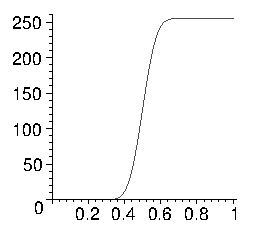
\includegraphics{fct}  \\
  Un carr\'e Noir et blanc & L'intensit\'e de gris \\
  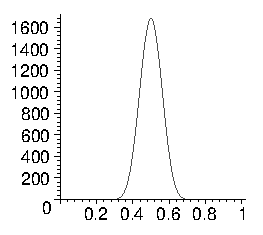
\includegraphics{Dfct}   &
  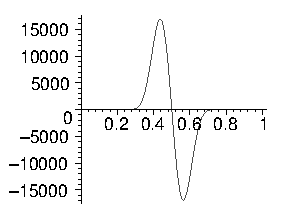
\includegraphics{DDfct}  \\
  La d\'eriv\'ee premi\`ere de l'intensit\'e & La d\'eriv\'ee seconde de l'intensit\'e \\
\end{tabular}
  \end{center}
\end{figure}
\par
Nous avons repr\'esent\'e dans la figure la variation de l'intensit\'e
de gris le long d'une ligne horizontale de ce carr\'e ainsi que les
d\'eriv\'ees premi\`ere et seconde de cette intensit\'e.
\par
On constate que le passage du blanc au noir s'accompagne d'une brusque
variation de l'intensit\'e. Mais afin de localiser plus pr\'ecis\'ement le
contour, nous pouvons aussi consid\'erer les d\'eriv\'ees~:
\begin{definition} ---
  Pour simplifier, on consid\`ere qu'un pixel fait partie d'un
  contour lorsque ce pixel correspond \`a un maximum de la vitesse de
  variation de l'intensit\'e i.e.\ lorsque~:
  \begin{itemize}
  \item la vitesse de variation de l'intensit\'e est maximale~;
  \item et l'acc\'el\'eration de la variation de l'intensit\'e est nulle.
  \end{itemize}
  En pratique, on se contente des conditions plus faibles~:
  \begin{itemize}
  \item la vitesse de variation de l'intensit\'e est au dessus d'un
    seuil~$v_{\mathrm{max}}$~;
  \item et l'acc\'el\'eration de la variation de l'intensit\'e est
    sous un seuil~$a_{\mathrm{min}}$.
  \end{itemize}
\end{definition}
\paragraph{Approximation discr\`ete des d\'eriv\'ees}
\subsection{Cas bidimensionnel}

\subsection{Travail \`a faire}
\end{document}

